\section{Classificazione dell'evento danneggiante}

Gli eventi danneggianti possono essere classificati in base ai costi
che possono comportare. Sono riportati in ordine crescente diverse categorie:

\begin{itemize}
\item \textbf{Negligible:} costo non significativo;
\item \textbf{Minor:} non ignorabile ma con costo senza impatto sul business;
\item \textbf{Major:} impatto su uno o più dipartimenti e può impattare sui
clienti esterni;
\item \textbf{Crisis:} evento che ci costa la permanenza sul mercato.
\end{itemize}

Questa classificazione non è semplice, anche perché ogni categoria ha una
classe di costi e contromisure diverse. Si può avere una sovrastima e una
sottostima dei costi, che portano rispettivamente ad un aumento eccessivo
dei costi o ad una sicurezza non adeguata.
Minor, major e crisis dovrebbero essere documentati e tracciati per poter
rimediare.

\subsection{Disastro e impatto}

Supponiamo di essere in un'università.
Potrebbero accadere i seguenti disastri:
\begin{itemize}
  \item Incendio: questo impatta sulle aule e il dipartimento. Come lo
  classifichiamo? Crisis, potrebbe essere major se limitato ad una parte del
  dipartimento. Attenzione: c'è la vita umana a rischio e quindi un forte
  rischio da tenere in considerazione;
  \item Attacco hacker: attaccano il sistema di registrazione dei voti. Può
  essere un evento major che ha implicazioni legali (non è possibile registrare
  voti);
  \item Indisponibilità dalla rete: livello di disastro, crisis. I dipartimenti
  dipendono dalla rete perché ci lavorano. Questo blocca completamente il
  dipartimento. Oggi una rete viene considerata come il sistema nervoso di un'
  organizzazione. Senza la quale l'organizzazione è costretta a fermarsi;
  \item Social engineering: può esserci un attacco al sistema di registrazione
  magari tramite una frode (mi prendono password e token);
  \item Server failure: collasso dei server. Si hanno le stesse conseguenze di
  network unavailable.
Classificato come major (crisi in alcuni casi, ad esempio durante una sessione
d'esami). Al giorno d'oggi è possibile contenere il disastro grazie a
contromisure standard, che richiedono un basso costo poiché basate su hardware.
\end{itemize}

\subsection{Recupero del servizio}

Per attuare un recupero del servizio è possibile che siano necessarie anche due
settimane.
Questo perché sono coinvolti processi che vanno capiti e contestualizzati.

\begin{figure}[h!]
        \begin{center}
                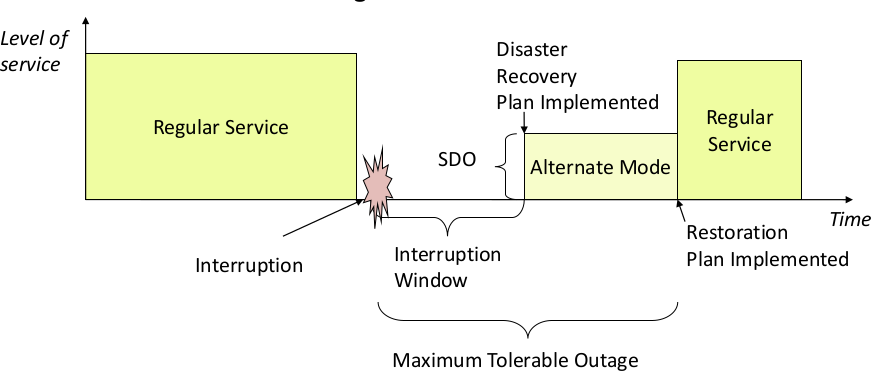
\includegraphics[scale=0.65]{res/img/recovery-times.png}
        \end{center}
        \caption{Grafico che mostra le fasi che portano dal servizio
        regolare, alla interruzione e infine al ripristino del servizio
        regolare, passando per il servizio degradato.}
        \label{fig:recovery-times}
\end{figure}

Prendiamo ora in esame la Figura \ref{fig:recovery-times}. In un primo 
momento abbiamo un servizio regolare. Quando si verifica un'interruzione
ci troviamo nell'\textbf{in\-ter\-rup\-tion win\-dow} (finestra di tempo 
in cui il servizio non è disponibile). Se è stato fatto un 
\textit{disaster recovery plan} possiamo entrare in 
\textbf{alternate mode} (servizio più limitato\footnote{Per 
esempio se prima era possibile servire 100 utenti contemporaneamente 
magari adesso \`e possibile servirne solamente 50.} ma disponibile).
La modalità alternativa si protrae fino a che non avviene la 
\textbf{restoration},
ovvero il ripristino del servizio regolare.

Il \textbf{Service Delivery Objective} è il livello di servizio che possiamo
fornire in \textit{alternate mode}: per esempio una banca vuole che sia
garantito almeno il 50\% delle transazioni durante la alternate mode, quindi
l'SDO è 50\%.

Il tempo passato tra l'inizio della modalità alternativa e il ripristino
del livello regolare di servizio viene definito come \textbf{Max\-i\-mum
Tol\-er\-a\-ble Out\-age} (MTO).

Può darsi che non sia possibile ritornare subito al 100\% dell'operatività.
È quindi necessario avere un \textbf{restoration plan} che permetta di passare
dall'\textit{alternate mode} al \textit{regular service mode} nel minor tempo
possibile.

La \textbf{Business Continuity} consiste nel riuscire ad offrire i
servizi \emph{critici} in caso di interruzioni.
La \textbf{Disaster Recovery} permette di sopravvivere anche se il
servizio IT è non disponibile.
Il \textbf{Disaster Recovery Plan} (DRP) è il piano che permette di passare in
modalità alternata.

\section{Classificazione dei servizi}\label{sec:classificazioneServizi}

Il servizio ha un costo associato, di conseguenza anche la mancata erogazione
del servizio lo ha. In ordine di importanza:
\begin{enumerate}
 \item \textbf{Critical:} non posso sostituirlo con un processo non IT, non si
deve fermare (p. es. telemedicina, un medico sta al MIT e tramite telemedicina
opera qualcuno a Ginevra, chiaramente il servizio non può essere interrotto).
Questo servizio implica la \textit{safety}. Ogni servizio che
implica la safety è critico per definizione;
 \item \textbf{Vital:} andare avanti a mano per un tempo molto ridotto. Costo
elevato;
 \item \textbf{Sensitive:} posso sostituire all'IT una procedura manuale per un
periodo limitato di tempo ma mi costa di più;

 \item \textbf{Nonsensitive:} posso andare avanti manualmente per un periodo
esteso di tempo.

\end{enumerate}

Nelle aziende di solito è sempre presente un processo critico. È strano se non
ce n'è neanche uno, ma dipende molto dalla realtà.

\subsection{Esempio: determinazione di criticità nei processi di business}

\begin{figure}[H]
 \centering
 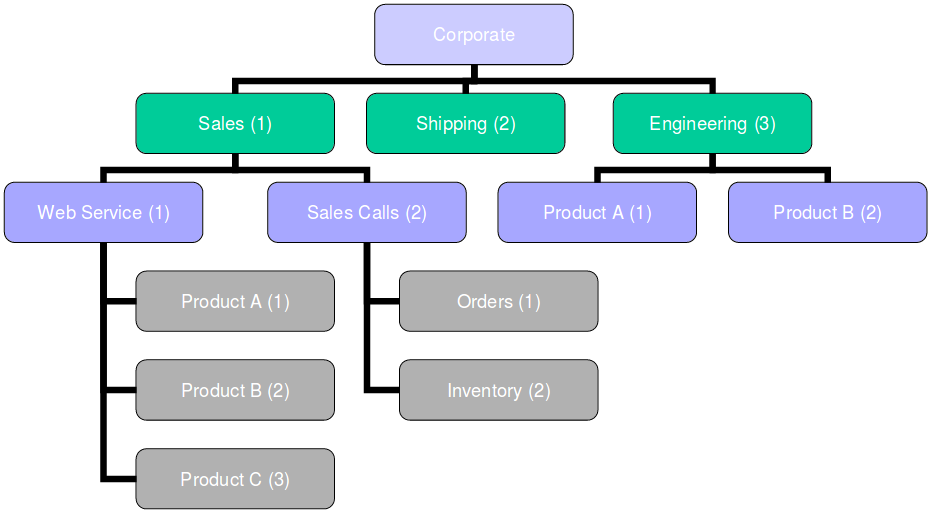
\includegraphics[scale=0.42]{dcobp}
 \caption{Una grande compagnia con le seguenti sotto-componenti}
\end{figure}

Il servizio più importante è \textit{sales}, perché non si può spedire senza
vendere. Per tutte le aziende le vendite sono critiche perché altrimenti non
fatturano.

Sotto alle sales abbiamo \textit{web service} and \textit{sales calls}. Tra i
due, \textit{web service} è critico perché non può essere sostituito
manualmente, mentre le \textit{sales calls} possono essere segnate a mano.

Gli ingegneri sono a bassa priorità perché anche se non lavorano per una
settimana sullo sviluppo di un prodotto semplicemente viene ritardato di una
settimana. Ovviamente bisogna tenere in considerazione il fatto che se c'è una
\textit{deadline} vicina il rischio sale.

\subsection{RPO and RTO}

\begin{itemize}
 \item \textbf{Recovery Point Objective}: ammontare di dati che possiamo
perdere quando recuperiamo dal backup;

 \item \textbf{Recovery Time Objective}: tempo che serve per recuperare le
applicazioni e ripartire in modo da poter ripristinare il servizio;

 \item \textbf{Orphan data}: dati che vanno persi e non sono recuperabili.
\end{itemize}

Se voglio avere \textit{RPO} basso devo avere una spesa maggiore (es. se lo
voglio minore vuol dire che devo effettuare backup più spesso, che significa
rendere non disponibile il dato su cui sto effettuando backup, ossia chi deve
lavorarci non può farlo).
\textit{RTO} è ovvio invece: più velocemente vogliamo essere operativi più
questo costa.

\subsection{Business Impact Analysis Summary}

Per fare un riassunto dell'unità viene qui proposto un esempio. In una
università, potremmo avere il seguente \textit{Business Impact Analysis
Summary}\footnote{Per comodità esiste anche l'abbreviazione BIA.}

\begin{table}[H]
\centering
\resizebox{\textwidth}{!}{%
\begin{tabular}{|l|l|l|l|p{5cm}|}
\hline
\textbf{Servizio}      & \textbf{RPO (ore)} & \textbf{RTO (ore)} &
\textbf{Risorse critiche}           & \textbf{Note speciali}

                           \\
\hline
Registrazione & 0 ore     & 4 ore     & SOLAR, rete, Registratore  & Alta
priorità durante Nov - Gennaio, Maggio - Giugno, Agosto \\
\hline
Personale     & 2 ore     & 8 ore     & PeopleSoft                 & Potrebbe
operare manualmente per alcune ore                  \\
\hline
Insegnamenti  & 1 giorno  & 1 ora     & D2L, rete, file di facoltà & Durante il
semestre scolastico: alta priorità               \\
\hline
\end{tabular}%
}
\caption{Un esempio di BIA per una Università}
\end{table}


\section{Tipologie di disaster recovery}

\subsection{RAID}

Sistema di ridondanza per i dati. Sono sei con diverse modalità.
\begin{itemize}
  \item RAID 0: i dischi anziché essere memorizzati su un disco sono
  memorizzati su due dischi. Possibile accesso parallelo ma niente backup
  (striping);
  \item RAID 1: backup su un altro disco (mirroring);
  \item Altri raid;
  \item RAID 5: si fa striping e redundancy. Ho più dischi e faccio striping
  con in aggiunta dei bit di parità.
\end{itemize}

\subsection{Network Disaster recovery}

Per recuperare un problema di rete la cosa più semplice è diversificare (avere
ridondanza, una rete alternativa). Due tipi di ridondanza:
\begin{itemize}
  \item \textbf{Alternative routing}: faccio un contratto con una società che
  mi fornisce un altro mezzo fisico che esce dalla mia azienda. Bisogna essere
sicuri che il mezzo che fornisce questa seconda società non sia lo stesso mezzo
fisico, altrimenti è inutile.
  \begin{itemize}
    \item last-mile circuit protection: se mi tranciano l'ultimo miglio tra
l'azienda e la centralina posso mantenere comunicazioni tramite
\textit{microwave communication}\footnote{Comunicazione a Microonde.}, faccio
comunicazione punto punto. Questa tecnologia viene usata abbastanza spesso in
quanto non richiede una particolare installazione ed è abbastanza economica;
    \item long-haul network diversity;
  \end{itemize}
  \item \textbf{Diverse routing}: si fa con la stessa società ma questa società
garantisce un instradamento diverso.
\end{itemize}

\subsection{Rottura vs Costi di ripristino}

Questi due obiettivi sono ovviamente conflittuali.

\begin{figure}[H]
  \centering
  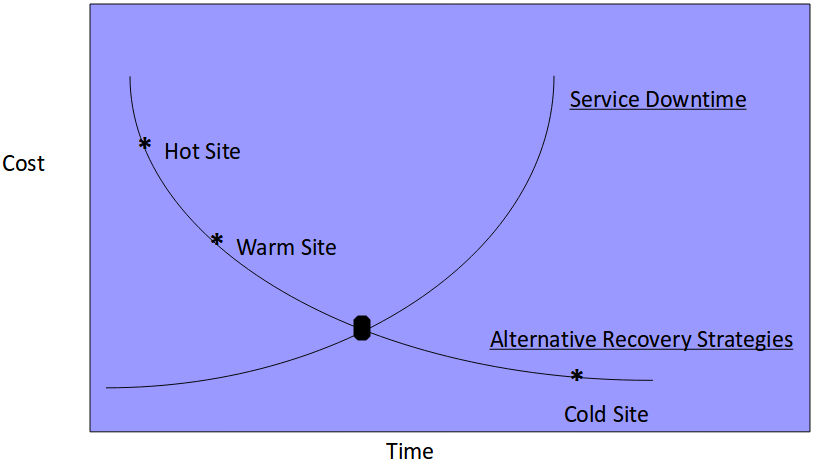
\includegraphics[scale=0.45]{dvsrc}
  \caption{Relazione tra tempo di disservizio e i costi di ripristino del
  servizio}
\end{figure}

Esistono diverse tecnologie di backup:
\begin{itemize}
  \item \textbf{Hot site}: il centro di \textit{backup} è allineato con il
  centro operativo (es. gestione dei satelliti, ho due siti, uno hot e l'altro
  operativo). Il tempo di recupero da \textit{downtime} è molto basso ma il
  costo è molto alto. Il costo è molto alto perché bisogna duplicare
  l'infrastruttura e il costo dell'\textit{information processes};
  \item \textbf{Warm site}: c'è un altro sito che ha tutti gli asset pronti
  per lavorare ma non è ancora operativo;
  \item \textbf{Cold site}: abbiamo un sito predisposto per l'emergenza ma che
  di fatto è vuoto. Ad esempio gli attacchi per il computer sono pronti ma
  mancano i server e le configurazioni. Questa installazione è quella che
  richiede più tempo per diventare operativa, anche se il suo costo è molto
  basso;
  \item Le \textbf{alternative recovery strategies} che hanno costi molto bassi
  di recupero ma si trovano in una fascia operativa media. Due società nello
  stesso segmento di mercato ma non troppo in competizione si potrebbero
  accordare per condividere i siti caldi. Questo rientra nella fase di
  \textbf{reciprocal agreeement};
  \item \textbf{Mobile site}: un mezzo mobile viene con un'antenna sul sito e
  garantisce la connettività.
\end{itemize}


\subsection{Cloud computing}

Il \textit{cloud computing} è caratterizzato da elasticità e scalabilità. Posso
scalare le risorse che mi servono, sia in positivo che in negativo perché non
sono regolari. Permette ad un'azienda di liberarsi del proprio reparto macchine
(no server fisici in loco).

\paragraph*{Vantaggi} Agilità, efficienza del costo, \textit{deployment} veloce
e alta scalabilità.

\paragraph*{Svantaggi} Costi customizzati, usabilità, connettività (mia e di
chi fornisce il \textit{cloud computing}), sicurezza.


\begin{figure}[H]
 \centering
 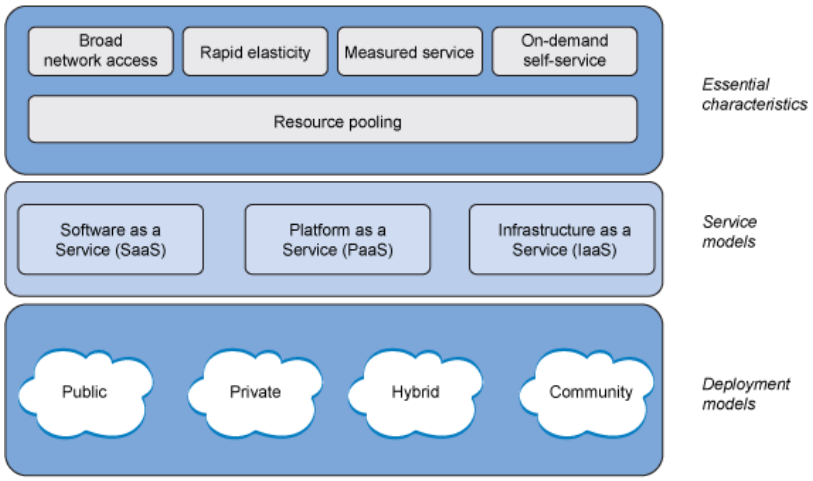
\includegraphics[scale=0.45]{itc}
 \caption{Una visione generale di come funziona un servizio \textit{cloud}}
\end{figure}

\subsubsection{Modello di dispiegamento}

Esistono diversi metodi di dispiegamento
\begin{itemize}
  \item Pubblico: pago e accedo al cloud (es. Amazon AWS);
  \item Privato: creo un mio \textit{datacenter} e lo utilizzo per i miei
  servizi (es. il datacenter di una banca);
  \item Ibrido: via di mezzo tra public e private;
  \item Comunitario: raggruppa organizzazioni che hanno lo stesso tipo di
  interessi o problematiche. Privato ma ``allargato''.
\end{itemize}

Da tenere sempre d'occhio è la sicurezza di questi servizi: quando si usa il
\textit{cloud} do i miei dati in mano a terzi. Un altro problema è la
\textit{multi tenancy}, ovvero quando vengono eseguiti più servizi di entità
diverse sulla stessa macchina grazie alla virtualizzazione. In caso di
fallimento di una macchina potrebbero fallire più servizi di diversi utenti,
per non parlare del fatto che un utente malintenzionato potrebbe tentare di
accedere al servizio di un altro utente risiedente sulla stessa istanza.

\subsubsection{Modello di servizio}

Esistono diversi modelli di servizio
\begin{itemize}
  \item Software (SaaS): si fa girare applicazioni di terze parti sul cloud.
  \item Platform (PaaS): viene fornito il sistema e l'ambiente di sviluppo, ci
  faccio girare le mie applicazioni.
  \item Infrastructure (IaaS): viene fornita la macchina e l'azienda ci mette
  sopra quello di cui ha bisogno.
\end{itemize}

\subsubsection{Caratteristiche essenziali}

Le caratteristiche essenziali che un servizio cloud offre sono: resource
pooling, broad network access, rapid elasticity, measured service e on-demand
self-service.

\subsubsection{Major Areas of Security Concerns}

\begin{itemize}
 \item \textbf{Service Level Agreement (SLA)}: definisce performance,
sicurezza, policy, disponibilità e molte altre cose. Esempio: contratto di
fornitura di internet, il SLA di solito è la banda minima garantita.
 \item Si ha \textbf{Multi-tenancy} quando l'applicazione è sullo stesso server
usato da altre organizzazioni. È quindi necessario avere un'adeguata
segmentazione e isolamento. Un set di \textit{policy} sono anche necessarie.
 \item \textbf{Your coverage}: la sicurezza dipende dall'infrastruttura
dell'azienda e da quella del cloud provider.
\end{itemize}

Non è possibile trasferire la responsabilità dei servizi nei confronti dei
propri clienti. Ad esempio: dichiarazione dei redditi con il commercialista, il
commercialista fa la dichiarazione ma chi la firma è il responsabile legale.

\subsubsection{Accordo reciproco}

\paragraph*{Vantaggi} Costo basso.

\paragraph*{Svantaggi} La sicurezza. Processi veramente critici vanno posti a
distanza geografica perché se capita una catastrofe è molto probabile che venga
colpito anche a chi è vicino (ovvero è presente una suscettibilità allo stesso
disastro).
